\documentclass[aspectratio=169, 12pt, handout]{beamer}


\usepackage{booktabs}
\usepackage{color}
\usepackage{ulem}
\usepackage{hyperref}
\usepackage{sidecap}
\usepackage{epstopdf}
\usepackage{enumerate}
\usepackage{bbm}
\usepackage{caption}
\usepackage{subfig}
\usepackage{multicol}
\usepackage{lmodern}
\usepackage{lipsum}
\usepackage{babel}
\usepackage{marvosym}
\usepackage{booktabs}
\usepackage{changepage}
\usepackage{natbib}
\usepackage{eurosym}
\usepackage{cancel}
\usepackage{pifont}
\usepackage{graphicx}
\usepackage{bbm}
\usepackage{amsmath}
\usepackage{textcomp}
\usepackage{comment}
\usepackage{listings}
\usepackage{xcolor}
\usepackage{inconsolata}
\usepackage{tikz}
\usetikzlibrary{shapes, arrows, positioning}

\lstset{
    language=Python,
    basicstyle=\ttfamily\footnotesize,
    keywordstyle=\color{blue},
    commentstyle=\color{gray},
    stringstyle=\color{teal},
    showstringspaces=false,
    breaklines=true,
    frame=single
}

\newcommand{\backupbegin}{
   \newcounter{framenumberappendix}
   \setcounter{framenumberappendix}{\value{framenumber}}
}
\newcommand{\backupend}{
   \addtocounter{framenumberappendix}{-\value{framenumber}}
   \addtocounter{framenumber}{\value{framenumberappendix}} 
}



\newenvironment{wideitemize}{\itemize\addtolength{\itemsep}{11pt}}{\enditemize}


\DeclareOptionBeamer{compress}{\beamer@compresstrue}
\ProcessOptionsBeamer

\mode<presentation>

\useoutertheme[subsection=false,shadow]{miniframes}
\useinnertheme{circles}

\beamertemplatenavigationsymbolsempty

\setbeamertemplate{footline}[frame number]
%\setbeamertemplate{headline}{} 

\setbeamercolor{section in toc shaded}{fg=gray}

% 2) choose your normal color for the current section:
\setbeamercolor{section in toc}{fg=black}  

% 3) hook a TOC frame at each new section
\AtBeginSection[]{
\addtocounter{framenumber}{-1}
  \begin{frame}[plain]
    \centering
    \tableofcontents[
      hideallsubsections,
      sectionstyle=show/shaded,    % “show” = current; “shaded” = others
      sectionstyle=show/shaded,
      currentsubsection,           % if you want sub‐levels, too
      currentsection
    ]
  \end{frame}
}
\setbeamersize{text margin left=5mm, text margin right=5mm}

\begin{document}

\title{Understanding Demand Estimation Methods}
\author{Presenter: Liyu Zhao}

\date{\today}

%TITLE FRAME
%%%%%%%%%%%%%%%%%%%%%%%%%%%%%%%%%%
\begin{frame}
%%%%%%%%%%%%%%%%%%%%%%%%%%%%%%%%%%
  \titlepage

\end{frame}


\section{Introduction}
\begin{frame}{The Big Picture: What is Demand Estimation?}
    The Data We See:
    \begin{itemize}
        \item Market Shares (Sales), Prices, Product Characteristics.
    \end{itemize}

    \vspace{0.3cm}
    The Questions We Want to Answer:
    \begin{itemize}
        \item Price Elasticity: If Tesla cuts prices by \$5,000, how many buyers will switch from BMW?
        \item New Product: If Apple releases a foldable iPhone, what will its market share be?
        \item Policy: If we tax sugary drinks, will consumers switch to diet soda or water?
    \end{itemize}

    \vspace{0.3cm}
    \textbf{The Challenge:}
    We need a model that links observed data to consumer choices.
\end{frame}

\begin{frame}{How to Model Consumer Choice?}
   Traditional (Continuous):
    \begin{itemize}
        \item ``I buy 3.5 liters of gasoline.'' (Continuous Quantity)
        \item Model: $\log Q = \alpha - \beta \log P + \epsilon$
    \end{itemize}

    \vspace{0.3cm}
    Discrete Choice (Reality for many markets):
    \begin{itemize}
        \item ``I buy either a Toyota or a Honda.'' (Mutually Exclusive)
        \item Consumers choose the product that gives the highest utility.
    \end{itemize}

    \vspace{0.2cm}
    \begin{block}{The Utility Framework}
        \[ U_{ij} = \underbrace{V_{ij}(\text{Price, Quality})}_{\text{Observed}} + \underbrace{\varepsilon_{ij}}_{\text{Unobserved Idiosyncratic Taste}} \]
        Consumer $i$ chooses product $j$ if $U_{ij} > U_{ik}$ for all $k$.
    \end{block}
\end{frame}


\begin{frame}{Why Structural Demand Estimation?}
    Why not just run a regression: $\ln(\text{Share}) = \alpha - \beta \text{Price}$?

    \vspace{0.3cm}
    \begin{itemize}
        \item \textbf{The Endogeneity Problem:}
        \begin{itemize}
            \item High price $\neq$ Low demand. (e.g., iPhone is expensive but popular).
            \item Reason: Unobserved quality ($\xi$) drives both price and demand. We need IVs.
        \end{itemize}
        
        \item \textbf{Supply-Side Inference:}
        \begin{itemize}
            \item From demand estimates, we can "back out" marginal costs without seeing accounting data.
        \end{itemize}
        
        \item \textbf{Counterfactuals:}
        \begin{itemize}
            \item Regression describes history. Structural models simulate the future (e.g., merger simulation).
        \end{itemize}

        \item \textbf{Basis for other analysis:}
        \begin{itemize}
            \item Vertical relations, network effects, consumer search, and many other...
        \end{itemize}
    \end{itemize}
\end{frame}



\begin{frame}{Why Mixed Logit \& BLP?}
    Standard Logit imposes strong restrictions on consumer behavior, leading to unrealistic predictions.
    \vspace{0.3cm}
    \begin{itemize}
        \item \textbf{The Limitation: Rigid Substitution Patterns}
        \begin{itemize}
            \item In Standard Logit, if a luxury car (e.g., BMW) raises its price, the model predicts consumers will switch to all other cars proportionally (even cheap ones like Fiat).
            \item Reality: They should switch to other luxury cars (e.g., Mercedes).
        \end{itemize}
        \vspace{0.3cm}
        \item \textbf{The Solution: Modeling Heterogeneity (Random Coefficients)}
        \begin{itemize}
            \item We allow consumers to have different tastes for characteristics (e.g., some love performance, some care about price).
            \item Result: High-income consumers stick to luxury goods; Price-sensitive consumers stick to budget goods. This naturally fixes the substitution problem.
        \end{itemize}
    \end{itemize}
\end{frame}

\begin{frame}{Learning From Replication}
    I replicated two influential papers, both of which were job market papers:
    \begin{itemize}
        \item ``Inference and Impact of Category Captaincy'', Management Science (Zhu, 2024)
        \item ``Advertising and Demand for Addictive Goods'', Marketing Science (Tuchman, 2019)
    \end{itemize} 
    
    \vspace{0.2cm}
    \textbf{Why is replication crucial?}
    \begin{itemize}
        \item Bridge the gap: Learn to translate abstract equations into executable code.
        \item Build your codebase: No need to start from scratch when launching your own project.
        \item Generate new ideas: Identifying limitations in existing code often leads to improvements and new research questions.
    \end{itemize}
    
    \vspace{0.2cm}
    \begin{block}{Resource Availability}
        Replication packages are increasingly available on top journals' websites.
    \end{block}
\end{frame}

\section{Mixed Logit}
\begin{frame}{The Foundation: Discrete Choice Framework}
    The Choice Setting
    \begin{itemize}
        \item Consumer $i$ faces a set of $J$ mutually exclusive alternatives (e.g., Coke, Pepsi, Sprite, Outside Option).
        \item Decision: Choose $j$ if and only if $U_{ij} > U_{ik}, \forall k \neq j$.
    \end{itemize}

    We decompose utility into an observed part ($V_{ij}$) and an unobserved shock ($\varepsilon_{ij}$):
    \[
        U_{ij} = \underbrace{V_{ij}}_{\text{Deterministic (e.g., } X_j\beta - \alpha p_j)} + \underbrace{\varepsilon_{ij}}_{\text{Random Shock}}
    \]

    To make this tractable, we assume $\varepsilon_{ij}$ follows an i.i.d. Type I Extreme Value (Gumbel) distribution.
    \begin{itemize}
        \item Why? It yields a closed-form solution for probabilities.
    \end{itemize}
\end{frame}

\begin{frame}{The Plain Logit Model (McFadden, 1974)}
    Under the Gumbel assumption, the probability of choosing $j$ has a beautiful closed-form expression:

    \[
        P_{ij} = \frac{\exp(V_{ij})}{\sum_{k=0}^J \exp(V_{ik})}
    \]

    \textbf{Key Features:}
    \begin{itemize}
        \item 0 to 1 bounded: Automatically behaves like a probability.
        \item Analytically tractable: Market shares ($s_j$) are easy to compute.
        \item Global convexity: The likelihood function is globally concave (easy to estimate).
    \end{itemize}
\end{frame}


\begin{frame}{The Limitation: Independence of Irrelevant Alternatives (IIA)}
    \textbf{The Definition:}
    The ratio of probabilities between any two goods ($A, B$) depends only on $A$ and $B$, not on the existence of a third good $C$.
    \[ \frac{P_A}{P_B} = \frac{e^{V_A}}{e^{V_B}} \quad (\text{Independent of } V_C) \]

    \textbf{The ``Red Bus / Blue Bus" Paradox}
    \begin{itemize}
        \item Scenario 1: Drive (6 people) vs. Red Bus (6 people). Ratio = 1:1.
        \item Scenario 2: Add a Blue Bus (identical to Red Bus).
        \item Logic Prediction (IIA): Ratio of Drive/Red Bus must stay 1:1.
        \item Result: Drive (4 people), Red Bus (4 people), Blue Bus (4 people).
        \item Reality: Drive (6 people), Red Bus (3 people), Blue Bus (3 people).
    \end{itemize}
    
    \textbf{Consequence:} Plain Logit forces proportional substitution. It cannot capture that Red Bus and Blue Bus are closer substitutes!
\end{frame}


\begin{frame}{Breaking the IIA}
    Plain Logit is restricted by IIA. How do we relax it? \\
    \textbf{1. Nested Logit}
    \begin{itemize}
        \item Idea: Group similar alternatives into ``nests'' (e.g., Sedan, SUV, No Purchase).
        \item Pros: Closed-form solution; easy to estimate.
        \item Cons: You must pre-specify the nests. The substitution pattern is ad-hoc, not found by the data.
    \end{itemize}

    \textbf{2. Multinomial Probit}
    \begin{itemize}
        \item Idea: Assume $\varepsilon \sim N(0, \Sigma)$. Allows flexible covariance.
        \item Pros: Theoretically flexible.
        \item Cons: Computationally intractable (requires high-dimensional integration).
    \end{itemize}

    \textbf{3. Mixed Logit / Random Coefficients}
    \begin{itemize}
        \item Idea: Allow $\beta$ to vary across individuals ($\beta_i = \bar{\beta} + \sigma \nu_i$).
        \item Theorem: McFadden \& Train (2000) proved that Mixed Logit can approximate any random utility model.
    \end{itemize}
\end{frame}

\begin{frame}{Mixed Logit}
    The utility of consumer $i$ choosing product $j$ is:
    \[
    u_{ij} = x_j \beta_i + \varepsilon_{ij} = \underbrace{x_j \beta}_{\text{mean utility}}+\underbrace{\sum_{k}x_{jk} \, \sigma_k\,\nu_{ik}}_{\text{heterogeneity}} + \underbrace{\varepsilon_{ij}}_{\text{iid T1EV}} (\text{Here, } \beta_i \sim N(\beta, \sigma^2))
    \]
    \vspace{0.3cm}
    Conditional on individual tastes $\nu_i$, the probability is:
    \[
        p_{ij}(\nu_i) = \frac{\exp(x_j \beta+x_j \,\sigma\,\nu_i)}{1 + \sum_{k=1}^J \exp(x_k \beta+x_k\,\sigma\,\nu_i)}
    \]

    \vspace{0.3cm}
    We observes choices $y_{ij}$ ($=1$ means \(i\) chooses \(j\)). The log-likelihood function is 
    \[
    LL(\{\beta,\sigma\}) = \sum_{i=1}^N \log \int \left( \prod_{j=1}^J p_{ij}(\nu)^{y_{ij}} \right) \phi(\nu) d\nu
    \]
\end{frame}

\begin{frame}{Numerical Integration}
The goal is to maximize the likelihood, but it does not have a closed form since RCs follow a normal distribution.
    \vspace{0.2cm}
    
    How to do it?
    \begin{itemize}
        \item Think of the integral as an expectation: $E_{\nu}[P_{ij}(\nu)]$.
        \item By the Law of Large Numbers, the sample mean converges to the expectation.
    \end{itemize}

    \vspace{0.2cm}
    We simulate the integral:
    \begin{enumerate}
        \item Draw $R$ random values: $\nu_1, \dots, \nu_R \sim N(0, 1)$.
        \item Calculate probability for each draw: $P_{ij}(\nu_r)$.
        \item Take the average:
    \end{enumerate}
    \[
    SLL(\{\beta,\sigma\}) = \sum_{i=1}^N \log \left( \frac{1}{R} \sum_{r=1}^R \prod_{j=1}^J p_{ij}^{y_{ij}}(\nu_r)  \right)
    \]
\end{frame}


\begin{frame}{Numerical Integration}
    \begin{figure}
        \centering
        \includegraphics[width=0.7\linewidth]{simulation.jpg}
    \end{figure}
    To reduce the number of draws, we can use the Halton draw which covers space more uniformly. \(\text{Halton}(R=100) \approx \text{Random}(R=1000)\).
\end{frame}


\begin{frame}{MLE Is Not Consistent}
    Let's distinguish between two types of convergence. \\
    \vspace{0.2cm}
    \textbf{1. The Role of Sample Size ($N$)}
    As $N \to \infty$, the sample average converges to the expected value of the objective function (Law of Large Numbers):
    \[
        \frac{1}{N} \sum_{i=1}^N \ln \hat{P}_{i}(\theta) \xrightarrow{p} E_{data} \left[ \ln \hat{P}_{i}(\theta) \right]
    \]
    \vspace{0.2cm}
    \textbf{2. The Role of Simulation Draws ($R$)}
    However, because of Jensen's Inequality:
    \[
        E \left[ \ln \hat{P}_{i} \right] < \ln( E[\hat{P}_{ij}] ) = \ln P_{i}
    \]
    So, even with infinite data ($N \to \infty$), the estimator is not converging to the true value.
\end{frame}

\begin{frame}{$R \to \infty$ Can Restore Consistency}
    Taylor Expansion: approximating $\ln(\hat{P})$ around the true probability $P$:
    \[
        \ln(\hat{P}) \approx \ln(P) + \frac{1}{P}(\hat{P} - P) - \frac{1}{2P^2}(\hat{P} - P)^2
    \]
    Taking expectations on both sides ($E[\hat{P}] = P$):
    \[
        E[\ln(\hat{P})] \approx \ln(P) + 0 - \frac{1}{2P^2} \underbrace{Var(\hat{P})}_{\text{Simulation Variance}}
    \]

    Since $\hat{P}$ is an average of $R$ draws, $Var(\hat{P}) \propto \frac{1}{R}$.
    \[
        \text{Bias} \approx - \frac{C}{R} \xrightarrow{R \to \infty} 0
    \]
\end{frame}



\begin{frame}{Comparison: MLE vs. Method of Simulated Moments (MSM)}
    If MSLE is biased, why not use MSM?

    \begin{table}[]
    \centering
    \begin{tabular}{l|c|c}
    \hline
    \textbf{Property} & \textbf{MLE (Likelihood)} & \textbf{MSM (Moments)} \\ \hline
    \textbf{Objective} & $\max \sum \ln(\hat{P})$ & $\min \| \text{Data} - \text{Model} \|$ \\ \hline
    \textbf{Linearity} & Non-linear ($\ln$) & Linear Difference \\ \hline
    \textbf{Bias (Fixed $R$)} & Biased & Unbiased \\  \hline
    \textbf{Efficiency} & High (Cramer-Rao) & Lower \\ \hline
    \end{tabular}
    \end{table}

    \vspace{0.2cm}
    \textbf{Conclusion:}
    \[
    \mathrm{MSE}(\hat{\theta})
    = \underbrace{\left( \mathbb{E}[\hat{\theta}] - \theta \right)^2}_{\text{Bias}^2}
    + \underbrace{\mathbb{E}\!\left[ \left( \hat{\theta} - \mathbb{E}[\hat{\theta}] \right)^2 \right]}_{\text{Variance}}
    \]
    \begin{itemize}
        \item MSM is consistent for fixed $R$, but less efficient (less information is used).
        \item In practice, we prefer MLE with large $R$ (or Halton) because efficiency.
    \end{itemize}
\end{frame}





\begin{frame}{Specify Analytical Gradient}
    To maximize $f(x)$, we need to find a step $\Delta x$ such that $f(x+\Delta x) > f(x)$.
    \[
        f(x + \Delta x) \approx f(x) + \underbrace{\nabla f(x)^T \Delta x}_{\text{Must be negative}}
    \]
    Without $\nabla f(x)$, the algorithm relies on slow finite-difference guesses.

\end{frame}

\begin{frame}[label=gradient]{Deriving Gradient}
    Consider the simplest case, no simulation. Let $i$ choose product $j$. The Log-Likelihood is: \hyperlink{full}{\beamerbutton{Full derivation}}
    \[
    LL(\beta) = \ln P_{ij} = \ln\left(\frac{\exp(x_{ij}\beta)}{\sum_{k=0}^J \exp(x_{ik}\beta)}\right) = x_{ij}\beta - \ln \left( \sum_{k=0}^J \exp(x_{ik}\beta) \right)
    \]

    \vspace{0.1cm}
    Take the derivative w.r.t $\beta$:
    \begin{align*}
        \frac{\partial LL}{\partial \beta} &= x_{ij} - \frac{\partial}{\partial \beta} \ln \left( \sum_{k} e^{x_{ik}\beta} \right) \\
        &= x_{ij} - \frac{1}{\sum_{k} e^{x_{ik}\beta}} \cdot \sum_{k} \left( e^{x_{ik}\beta} \cdot x_{ik} \right) \quad \text{(Chain Rule)} \\
        &= x_{ij} - \sum_{k} \underbrace{\left( \frac{e^{x_{ik}\beta}}{\sum_{m} e^{x_{im}\beta}} \right)}_{P_{ik}(\beta)} \cdot x_{ik}
    \end{align*}
    
\end{frame}

\begin{frame}{Deriving Gradient}
    The gradient has a beautiful, intuitive form:
    
    \[
    \nabla_\beta LL = \underbrace{x_{ij}}_{\text{Observed Attribute}} - \underbrace{\sum_{k=1}^J P_{ik}(\beta) x_{ik}}_{\text{Expected Attribute } E[x]}
    \]

    \vspace{0.3cm}
    \textbf{Intuition:}
    \begin{itemize}
        \item Imagine $x$ is ``Horsepower''. I chose a Ferrari ($x_{high}$).
        \item If the model predicts I like slow cars, then $E[x]$ is low.
        \item Gradient $= x_{high} - x_{low} > 0$.
        \item \textbf{Action:} Increase $\beta_{\text{HP}}$. The model stimulates the preference for horsepower up until Observed $\approx$ Expected.
    \end{itemize}
    
    \footnotesize{This is essentially the Method of Moments condition!}
\end{frame}

\begin{frame}{Optimization Algorithms}
    Now we have the direction $\nabla LL$ (Gradient). How do we update $\beta$?
    
    \vspace{0.2cm}
    \textbf{1. Gradient Ascent: } Simple but slow.
    Just follow the steepest slope.
    \[ \beta_{new} = \beta_{old} + \alpha \cdot \nabla LL \]

    \vspace{0.2cm}
    \textbf{2. Newton's Method: } Fast but expensive to get \(H\)
    \[ \beta_{new} = \beta_{old} - \underbrace{H^{-1}}_{\text{Curvature}} \nabla LL \]


    \vspace{0.2cm}
    \textbf{3. Quasi-Newton / BFGS}
    \begin{itemize}
        \item \textbf{Idea:} Don't calculate $H$. Instead, approximate $H^{-1}$ using the history of gradients.
        \item \textbf{Result:} Speed of Newton + Low cost of Gradient Ascent.
        \item This is what \texttt{pyblp} and most solvers use by default.
    \end{itemize}
\end{frame}

\begin{frame}{The Remaining Bottleneck}
    Even with analytical gradients, estimation is slow. Why?
    
    \vspace{0.3cm}
    \begin{itemize}
        \item Heavy operations
        \begin{itemize}
            \item We perform matrix multiplication ($X\beta$) and exponentiation ($\exp$) for every consumer, every product, and every simulation draw.
            \item Tensor Size: $N (10^4) \times J (10) \times R (500) = 50 \text{ Million Operations}$.
        \end{itemize}     
        \vspace{10pt}
        \item The CPU limitation (sequential computing)
        \begin{itemize}
            \item \texttt{NumPy} runs primarily on the CPU.
            \item CPUs have few cores (8-16). They process large matrices in ``chunks'' (sequentially).
        \end{itemize}
    \end{itemize}

\end{frame}

\begin{frame}{Why PyTorch?}
    PyTorch is not just for neural networks. For structural estimation, it offers two advantages:
    
    \vspace{0.3cm}
    \begin{itemize}
        \item Massive parallel computation (GPU Acceleration)  (Later on this point!)
            \begin{itemize}
            \item Move data from CPU to GPU.
            \item GPUs have thousands of small cores.
            \item We can compute utility for all $N$ consumers and $R$ draws simultaneously.
        \end{itemize}
        \item Automatic Differentiation (AutoGrad)
            \begin{itemize}
            \item No need to manually derive the complex gradient.
            \item \texttt{loss.backward()} computes exact gradients using the computational graph.
        \end{itemize}
    \end{itemize}
\end{frame}


\begin{frame}{Backward Propagation}
    AutoGrad doesn't ``know'' the full formula. It just multiplies local gradients step-by-step.
    
    \begin{center}
    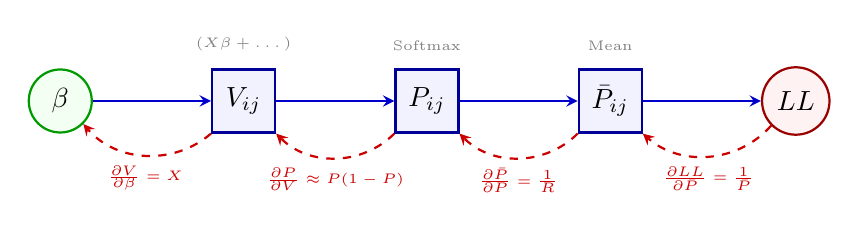
\begin{tikzpicture}[
        node distance=1.5cm,
        input/.style={circle, draw=green!60!black, fill=green!5, thick, minimum size=0.8cm},
        op/.style={rectangle, draw=blue!60!black, fill=blue!5, thick, minimum size=0.8cm},
        loss/.style={circle, draw=red!60!black, fill=red!5, thick, minimum size=0.8cm},
        arrow/.style={->, >=stealth, thick, color=blue!80!black},
        back/.style={->, >=stealth, dashed, thick, color=red!80!black}
    ]

    % --- Nodes (Forward Pass) ---
    \node[input] (beta) {$\beta$};
    % Utility (V)
    \node[op, right=1.5cm of beta] (utility) {$V_{ij}$};
    \node[above=0.1cm of utility, font=\tiny, color=gray] {$(X\beta + \dots)$};
    
    % Probability (P)
    \node[op, right=1.5cm of utility] (prob) {$P_{ij}$};
    \node[above=0.1cm of prob, font=\tiny, color=gray] {Softmax};

    % Integral (I)
    \node[op, right=1.5cm of prob] (integral) {$\bar{P}_{ij}$};
    \node[above=0.1cm of integral, font=\tiny, color=gray] {Mean};

    % Log-Likelihood (LL)
    \node[loss, right=1.5cm of integral] (ll) {$LL$};

    % --- Forward Edges (Blue) ---
    \draw[arrow] (beta) -- (utility);
    \draw[arrow] (utility) -- (prob);
    \draw[arrow] (prob) -- (integral);
    \draw[arrow] (integral) -- (ll);

    % --- Backward Edges (Red - Step-by-Step) ---
    % 1. LL -> Integral
    \draw[back, bend left=45] (ll) to node[below, font=\tiny] {$\frac{\partial LL}{\partial \bar{P}} = \frac{1}{\bar{P}}$} (integral);
    
    % 2. Integral -> Prob
    \draw[back, bend left=45] (integral) to node[below, font=\tiny] {$\frac{\partial \bar{P}}{\partial P} = \frac{1}{R}$} (prob);
    
    % 3. Prob -> Utility (Softmax Derivative)
    \draw[back, bend left=45] (prob) to node[below, font=\tiny] {$\frac{\partial P}{\partial V} \approx P(1-P)$} (utility);
    
    % 4. Utility -> Beta
    \draw[back, bend left=45] (utility) to node[below, font=\tiny] {$\frac{\partial V}{\partial \beta} = X$} (beta);

    \end{tikzpicture}
    \end{center}

    \vspace{0.2cm}
    \textbf{The Logic:}
    \[
        \underbrace{\frac{\partial LL}{\partial \beta}}_{\text{Goal}} = 
        \underbrace{\frac{\partial LL}{\partial \bar{P}}}_{\text{Step 1}} \cdot 
        \underbrace{\frac{\partial \bar{P}}{\partial P}}_{\text{Step 2}} \cdot 
        \underbrace{\frac{\partial P}{\partial V}}_{\text{Step 3}} \cdot 
        \underbrace{\frac{\partial V}{\partial \beta}}_{\text{Step 4}}
    \]
    \footnotesize{Each node only needs to know its own derivative. The computer just multiplies them together!}
\end{frame}

\begin{frame}[fragile]{Code Comparison}
    \begin{lstlisting}[language=Python, basicstyle=\ttfamily\scriptsize]
# Manual
def gradient(beta, sigma):
  # 1. Calc Shares (P)
  P = ... 
  
  # 2. Manual Formula
  grad_beta = X - (P @ X)
  
  return grad_beta

# AutoGrad
# Define params
beta = torch.tensor([2.0], requires_grad=True)

# 1. Forward Pass
LL = compute_LL(beta, ...)

# 2. Backward Pass
LL.backward()
    \end{lstlisting}
\end{frame}


\begin{frame}{Application: Advertising and Demand for Addictive Goods (Tuchman, 2019)}
    \textbf{Research Question: }Do E-cigarette ads decrease demand for traditional cigarettes? 
    
    \vspace{0.2cm}
    The Model: Mixed Logit with State Dependence (Addiction)
    
    Consumer $i$ chooses product $j$ at week $t$. Utility depends on past choices:
    \[
        U_{ijt} = \underbrace{\alpha p_{jt} + \phi A_{mt}}_{\text{Mean Utility}} + \underbrace{\gamma \mathbb{I}(y_{it-1}=j)}_{\text{Addiction (State Dep.)}} + \underbrace{\mu_{ij}}_{\text{Heterogeneity}} + \epsilon_{ijt}
    \]
    \begin{itemize}
        \item Data: Nielsen Household Panel.
        \item Key Challenge: We must estimate the random coefficients ($\sigma_{\beta}$) and addiction parameters ($\gamma$) by integrating over thousands of consumers.
    \end{itemize}

\end{frame}


\begin{frame}{Implementation Details: Coding the Likelihood}
    Before we compute gradients, the Forward Pass must be robust and efficient.
    
    \vspace{0.2cm}
    \textbf{1. The Panel Data Logic}
    \[ \text{Log-Likelihood} = \sum_i \ln \left( \frac{1}{R} \sum_r \underbrace{\left( \prod_t P_{ijt}(\nu_{ir}) \right)}_{\text{Product over Time}} \right) \]

    \vspace{0.2cm}
    \textbf{2. Fixed Random Draws }
    \begin{itemize}
        \item Draws ($\nu$) must be generated outside the optimization loop. If draws change every iteration, the optimizer fails to converge.
    \end{itemize}

    \vspace{0.2cm}
    \textbf{3. Numerical Stability (Log-Sum-Exp)}
    \begin{itemize}
        \item Calculating $e^{V}$ leads to overflow if $V$ is large.  Subtract $V_{max}$ before exponentiation: $\frac{e^{V_j - V_{max}}}{\sum e^{V_k - V_{max}}}$.
    \end{itemize}
\end{frame}


\begin{frame}{Why AutoGrad?}
    \begin{itemize}
        \item Model maintenance: If a reviewer asks, ``Is the addiction parameter $\gamma$ heterogeneous?''
        \begin{itemize}
            \item Manual: You must re-derive $\frac{\partial LL}{\partial \sigma_\gamma}$, update the gradient code.
            \item AutoGrad: Change 1 line in the Utility function. \texttt{loss.backward()} handles the rest
        \end{itemize}
        \item High-dimensional structure: 
        \begin{itemize}
            \item Deriving gradients through matrix operations (Cholesky, Inverse) is a nightmare of linear algebra.
            \item AutoGrad: Handles matrix calculus derivatives natively.
        \end{itemize}
    \end{itemize}
\end{frame}



\section{BLP}

\begin{frame}{Transition: From Micro-Data to Market-Level Data}
    We have seen how Mixed Logit handles heterogeneity using household panel data.
    
    \vspace{0.2cm}
    \textbf{But what if we only have aggregate data?}
    \begin{itemize}
        \item Data: Market shares ($s_{jt}$), Prices ($p_{jt}$), Characteristics ($x_{jt}$).
        \item No individual choices ($y_{ijt}$) are observed.
    \end{itemize}

    \vspace{0.3cm}
    \textbf{The ``Unobserved Quality'' Problem ($\xi_{jt}$)}
    \[
        u_{ijt} = \alpha_i p_{jt} + x_{jt}\beta_i + \underbrace{\xi_{jt}}_{\text{Unobserved Quality}} + \epsilon_{ijt}
    \]
    \begin{itemize}
        \item $\xi_{jt}$: Characteristics observed by consumers and firms (e.g., style, prestige), but unobserved by the econometrician.
        \item Endogeneity: Firms set prices based on $\xi_{jt}$ (High quality $\to$ High price).
        \item Result: $Corr(p_{jt}, \xi_{jt}) > 0$, which yields biased price elasticities.
    \end{itemize}
\end{frame}


\begin{frame}{The BLP Solution: GMM with Instrumental Variables}
    Berry, Levinsohn, and Pakes (1995) propose a solution to estimate mixed logit with aggregate data and endogenous prices.
    
    \vspace{0.3cm}
    \textbf{Key Idea: Inversion}
    \begin{itemize}
        \item We cannot use MLE because $\xi_{jt}$ is not random noise; it's correlated with price.
        \item Instead, we invert the market share function to recover the ``Mean Utility'' ($\delta_{jt}$):
        \[
            s_{jt}(\delta, \theta_{2}) = S_{jt}^{Data} \implies \delta_{jt}(\theta_2) = s^{-1}(S^{Data}, \theta_2)
        \]
    \end{itemize}
    
    \vspace{0.2cm}

    Once we recover $\delta_{jt}$, we have a linear equation:
    \[
        \delta_{jt} = x_{jt}\beta + \alpha p_{jt} + \xi_{jt}
    \]
    Now we can use IVs to handle the correlation between $p_{jt}$ and $\xi_{jt}$.
\end{frame}


\begin{frame}{Berry's Inversion (1994)}
    The market share (there is no RC):
    \[
        s_{jt} = \frac{\exp(x_{jt}\beta - \alpha p_{jt} + \xi_{jt})}{1 + \sum_{k} \exp(x_{kt}\beta - \alpha p_{kt} + \xi_{kt})}
    \]
    Normalize the outside utility to zero:
    \[
        s_{0t} = \frac{1}{1 + \sum_{k} \exp(\delta_{kt})}
    \]
    This implies
    \[
        \ln\frac{s_{jt}}{s_{0t}} = x_{jt}\beta - \alpha p_{jt} + \xi_{jt} 
    \]

      \textbf{Implication:} We can now estimate this using IV Regression (2SLS/GMM) to solve the correlation between $p_{jt}$ and $\xi_{jt}$.

\end{frame}

\begin{frame}{When There are Random Coefficients}
    The market share is the integral of individual probabilities over the population distribution $F(\nu)$:
    \[
        s_{jt}(\delta, \theta_2) = \int \frac{\exp(\delta_{jt} + \mu_{ijt})}{1 + \sum_{k} \exp(\delta_{kt} + \mu_{ikt})} \, dF(\nu)
    \]

    Here, \(\delta_{jt}=x_{jt}\beta-\alpha p_{jt}+\xi_{jt}\), and \(\mu_{ijt}=\sum_{k} x_{jtk} (\sigma_k \nu_{ik}) - p_{jt} (\sigma_p \nu_{ip}) \) 
    \vspace{0.2cm}
    
    Since the integral has no closed form, we approximate it by simulation (averaging over $R$ draws):
    \[
        s_{jt} \approx \frac{1}{R} \sum_{r=1}^R \frac{\exp(\delta_{jt} + \mu_{rjt})}{1 + \sum_{k} \exp(\delta_{kt} + \mu_{rkt})}
    \]
\end{frame}


\begin{frame}{Inner Loop: Contraction Mapping}
    Since we cannot analytically invert the integral $s_{jt}(\delta, \theta_2)$, we solve for $\delta$ numerically.
    
    \vspace{0.2cm}
    From Berry (1994), we use the following iteration:
    \[
        \delta_{jt}^{h+1} = \delta_{jt}^{h} + \ln(S_{jt}^{Data}) - \ln(s_{jt}(\delta^h, \theta_2))
    \]
    \vspace{-5pt}
    \begin{itemize}
        \item \textbf{Intuition:} Take \(\theta_2\) as given. Share is increasing in \(\delta\). If Model Share \(<\) Data Share, increase $\delta$.
        \item \textbf{Convergence:} \(T(\delta)=\delta+\ln(s)-\ln(s(\delta))\) is a contraction mapping (Berry, 1994).
    \end{itemize}

    \vspace{0.2cm}
    Connection to Rust's NFXP: BLP is structurally identical to John Rust's Nested Fixed Point algorithm.
    \[
    T(W(x)) = \max_{d} \left[ u(x, d; \theta)+ \beta \, E\!\left[ W(x') \mid x, d; \theta \right] \right]
    \]

\end{frame}


\begin{frame}{The Outer Loop: Estimating Parameters via GMM}
    Once the contraction mapping converges (\(|\delta_{jt}^{h+1}-\delta_{jt}^{h}| < \text{threshold}\)) for a given guess of non-linear parameters $\theta_2$, we obtain the mean utilities $\delta_{jt}(\theta_2)$.

    \begin{enumerate}
        \item Recover linear parameters \((\hat{\beta},\hat{\alpha})\) using 2SLS and the structural error ($\xi_{jt}$):
        \[
        \xi_{jt}(\theta) = \delta_{jt}(\theta_2) - (x_{jt}\hat{\beta} - \hat{\alpha} p_{jt})
        \]
        \item Create moment conditions: since price is endogenous ($E[\xi p] \neq 0$), we use Instruments $Z_{jt}$:
        \[
        \bar{g}(\theta) = \frac{1}{J \times T} \sum_{j,t} Z_{jt}' \xi_{jt}(\theta)
        \]
        \item GMM: we search for parameters $\hat{\theta}_2$ that minimize the distance of moments to zero:
        \[
        \min_{\theta_2} J(\theta_2) = \bar{g}(\theta_2)' W \bar{g}(\theta_2) = \xi(\theta_2)' Z W Z' \xi(\theta_2)
     \]
    \end{enumerate}
\end{frame}



\begin{frame}{Identification}
    Recall the moment conditions we used:
    \[
        E\!\left(\xi_{jt} X_{jt}\right) = 0,
        \qquad
        E\!\left(\xi_{jt} Z_{jt}\right) = 0.
    \]    
    $E\!\left(\xi_{jt} X_{jt}\right)=0$ are used to identify
    $\beta$. One of the $E\!\left(\xi_{jt} Z_{jt}\right)=0$ conditions
    (where $Z_{jt}$ is an IV for price) is used to identify $\alpha$. The identification of $\sigma$ comes from the
    rest of the $E\!\left(\xi_{jt} Z_{jt}\right)=0$ conditions.
    \vspace{0.2cm}
    
    \textbf{Types of instruments:}
    \begin{itemize}
        \item Cost shifters: Shift supply. Assume inputs aren't correlated with quality.
        \item Hausman IV: price of product \(j\) in other markets \(p_{j't}\): Shift prices via common costs. Assume no national demand shocks.
        \item BLP IV: characteristics of rival products \(x_{-j,t}\), and other variants: (Shift markups via competition intensity. Assume product characteristics are predetermined in the short run.)
        \begin{itemize}
            \item \(\sum_{j' \neq j}\left( X_{jtm} - X_{j',t,m} \right)^2\),   \(\sum_{j' \neq j}
        \left( X_{jtm} - X_{j',t,m} \right)
        \left( X_{jtm'} - X_{j',t,m'} \right)\)
        \end{itemize}
    \end{itemize}
\end{frame}


\begin{frame}{Identification}
    \textbf{Question:} What variations identify random coefficients? \\
    \textbf{Answer:} Substitution patterns - with random coefficients, consumers substitute more to a similar product. \\
    \vspace{0.2cm}
    Variations in substitution patterns:
    \begin{itemize}
        \item Substitution based on characteristic distance.
        \item Choice set variations.
    \end{itemize}

    Sometimes, there is not enough variation to identify the unobserved heterogeneity in the data. Instead, we can identify the heterogeneity correlated to demographics. It is easier to use observables to explain substitution patterns.
    \[
    \beta_i = \bar{\beta} + \underbrace{\Sigma\nu_i}_{\text{unobserved}}+ \underbrace{\Pi D_i}_{\text{demographics}}
    \]
\end{frame}


\begin{frame}{Application: Inference and Impact of Category Captaincy (Zhu, 2024)}
    This paper focuses on category captaincy, which is a vertical arrangement where retailers delegate shelf placement and pricing to a leading manufacturer. However, the contract is confidential. In the data, we can just see Dannon leads in some chains, Yoplait in others. Is this due to consumer preference or shelf advantage (better display, space)? \\
    \vspace{5pt}
    Utility of consumer $i$ for product $j$ at retailer $r$:
        \[
        u_{ijrmt}
=
\bar{u}\!\left( x_{jrmt}, \beta, \eta_{irmt} \right)
+ \xi_{jrmt}
+ \varepsilon_{ijrmt}
        \]
    \textbf{Key Innovation}: Decompose unobserved quality $\xi_{jrmt}$:
        $$ \xi_{jrmt} = \xi_{jt} + \underbrace{\xi_{brt}}_{\text{Captaincy Effect}} + \Delta \xi_{jrmt} $$
\end{frame}


\begin{frame}{Application: Inference and Impact of Category Captaincy}
        \textbf{Identification: }To solve price endogeneity, the paper uses two sets of IVs (selected using the specification test (Gandhi and Houde 2019) and Lasso (Belloni et al. 2012)):
        \vspace{0.2cm}
    \begin{itemize}
        \item \textbf{Cost Shifters}: cost or markup shifters, which includes input/transportation costs interacted with product characteristics, assortment variables, and demographic characteristics of a brand’s main market within retailer interacted with that brand’s product characteristics
        \vspace{0.1cm}
        \item \textbf{Differentiation IVs}: characterizes the degree of differentiation of each product in a retailer market and exploits variation in household demographics across retailer markets (Gandhi \& Houde, 2019).
    \end{itemize}
\end{frame}




\begin{frame}{\texttt{PyBLP}}
    The burdens of hand-coding BLP: updating the optimal weighting matrix, deriving the analytical Jacobian, and managing numerical stability with high-precision tolerances. \texttt{PyBLP} handles these burdensome steps. That's why I recommend it. \\
    \vspace{0.3cm}
    Aside from the estimation of BLP, it can also do post-estimation practices: price elasticities, consumer surplus calculation, markup and margin calculation, and merger simulation. \\ 
    \vspace{0.3cm}
    The estimation in \texttt{pyblp} is organized around three core objects:
Formulation, Integration, and Problem.

    
\end{frame}

\begin{frame}[fragile]{The Core Workflow in \texttt{PyBLP}}
\small
1. Model Configuration: separate linear parameters $(\beta, \alpha)$ from non-linear random coefficients $(\Sigma)$.

\begin{lstlisting}[language=Python, basicstyle=\ttfamily\footnotesize]
X1_formulation = pyblp.Formulation(
    '0 + prices + sugar + sodium + fat + size + # flavor + calorie + organic + # sales',
    absorb='C(fe_product_year) + C(fe_brand_retailer_year)'
)

X2_formulation = pyblp.Formulation(
    '1 + prices + # flavor + size + sodium + sugar + fat'
)

agent_formulation = pyblp.Formulation('0 + income + kids + edu')

\end{lstlisting}

\end{frame}


\begin{frame}[fragile]{The Core Workflow in \texttt{PyBLP}}
\small
2. Integration and Initialization: 
\begin{lstlisting}[language=Python, basicstyle=\ttfamily\footnotesize]
problem = pyblp.Problem(
    product_formulations=(X1_formulation, X2_formulation),
    product_data=product_data,
    agent_data=agent_data,
    agent_formulation=agent_formulation
)

results = problem.solve(
    sigma=initial_sigma, 
    sigma_bounds=(np.zeros((7, 7)), np.zeros((7, 7))),
    pi=initial_pi, pi_bounds=(pi_lower, pi_upper),
    optimization=pyblp.Optimization('l-bfgs-b', {'gtol': 1e-4}),
    method='2s', se_type='clustered'
)
\end{lstlisting}

\end{frame}


\section{Integrated Model}
\begin{frame}{Revisit Tuchman (2019)}
    \textbf{Problem:}
    \begin{itemize}
        \item Micro data alone: Sparse. Hard to estimate precise brand-market-time fixed effects ($\delta_{jmt}$) needed to control for price endogeneity.
        \item Macro data alone: Hard to identify complex heterogeneity distributions ($\Sigma$) and state dependence parameters ($\gamma$).
    \end{itemize}
    
    \textbf{Solution:}
    \begin{itemize}
        \item Use aggregate data to pin down mean utilities ($\delta_{jmt}$).
        \item Use household data to identify non-linear parameters ($\Sigma, \gamma$).
        \item Consistency Constraint: The $\delta_{jmt}$ that rationalizes aggregate shares must be the same $\delta_{jmt}$ entering the household likelihood.
    \end{itemize}
\end{frame}

\begin{frame}{The Estimation Algorithm}
    We iterate between two steps until convergence of non-linear parameters $\theta_2 = \{\Sigma, \gamma\}$:
    
    \vspace{0.5cm}
    \textbf{Step 1: The Macro Step (Contraction Mapping)}
    \begin{itemize}
        \item Given $\theta_2$, solve for $\delta_{jmt}$ such that $s^{pred}(\delta, \theta_2) = s^{obs}$.
        \item Challenge: Standard BLP is parallel over markets ($t$ is independent). Tuchman's model is recursive: Market shares at $t$ depend on market shares $t-1$.
    \end{itemize}
    
    \vspace{0.3cm}
    \textbf{Step 2: The Micro Step (MLE)}
    \begin{itemize}
        \item Treat $\delta_{jmt}$ as data (fixed).
        \item Maximize $LL(\theta_2 | \delta, \text{Household Data})$.
    \end{itemize}
    
    \vspace{0.3cm}
    \textbf{Step 3: Linear Parameters (Post-Convergence)}
    \begin{itemize}
        \item Regress converged $\delta_{jmt}$ on Prices/Ads (Border strategy).
    \end{itemize}
\end{frame}

\begin{frame}[fragile]{Step 1: Handling Recursion with Numba}
    \[ s_{jmt} = \int \sum_{k} \pi_{jmt}(k) \cdot \underbrace{\Pr(y_{it-1}=k)}_{\text{Evolves over time!}} dF(\beta) \]
    
    \textbf{Implementation Detail:}
    \begin{itemize}
        \item Cannot vectorize over $T$. We must loop $t=1 \dots T$.
        \item Pure python loops are too slow for the contraction mapping.
        \item \textbf{Solution:} \texttt{@jit(nopython=True)} compiles the recursion to machine code.
    \end{itemize}

    \begin{lstlisting}[language=Python, basicstyle=\ttfamily\tiny]
# Core logic inside Numba
for t in range(T):
    if t > 0:
        delta_t = delta_sol[t-1, :, :].copy() # History dependence
    
    # Contraction Mapping Loop for current t
    while error > 1e-9:
        # ... solve for delta_t ...
        
    # Update state distribution for t+1
    prob_state_lag = update_probs(probs)
    \end{lstlisting}
\end{frame}


\begin{frame}[fragile]{Comparison}
    \begin{lstlisting}[language=Python, basicstyle=\ttfamily\tiny]
import time
import numpy as np
from numba import jit

data = np.arange(1_000_000)
# Loop
result = []
for x in data:
    result.append(x**2) # 0.0493s

# Vectorization
result = data ** 2 # 0.0091s

# Numba
@jit(nopython=True, cache=True)
def square_loop(data):
    result = np.empty(len(data))
    for i in range(len(data)):
        result[i] = data[i] ** 2
    return result

_ = square_loop(data) # First time: 0.0377s
_ = square_loop(data) # After compilation: 0.0008s

    \end{lstlisting}
\end{frame}

\begin{frame}[fragile]{Step 2: GPU Acceleration with PyTorch}
    \[ LL = \sum_i \ln \int \prod_t P_{ijt}(\delta_{jmt}, \gamma, \Sigma) dF(\nu) \]
    
    \textbf{Implementation Detail:}
    \begin{itemize}
        \item We need to broadcast the $\delta_{jmt}$ (solved in Step 1) to thousands of households.
        \item This involves massive matrix operations: $(N_{HH} \times T \times R_{draws})$.
        \item \textbf{Solution:} Move tensors to GPU.
    \end{itemize}

    \begin{lstlisting}[language=Python, basicstyle=\ttfamily\tiny]
# Broadcasting Macro delta to Micro observations
t_delta_i = t_delta_est[self.t_h_week, self.t_h_mkt, :].unsqueeze(2)

# Adding Heterogeneity (Sigma) and Addiction (Gamma)
t_U = t_delta_i + t_mu_matrix + t_lag_boost

# Choice Probabilities computed in parallel on GPU
t_exp_U = torch.exp(t_U)
    \end{lstlisting}
\end{frame}

% Slide 6: Handling Initial Conditions (The Burn-in)
\begin{frame}{Handling Initial Conditions: The Burn-in Period}
    \textbf{Issue:}
    \begin{itemize}
        \item At $t=0$, we don't know the distribution of addicted users.
        \item Assuming an arbitrary starting distribution (e.g., all non-smokers) biases the early estimates.
    \end{itemize}
    
    \textbf{Solution in Code:}
    \begin{itemize}
        \item Simulate the first 24 weeks without using them in the likelihood.
        \item Start from a steady state:
    \end{itemize}
    \begin{equation*}
       LL(\theta) = \sum_{t=\text{burn\_in}}^T \ln P(y_{it} | y_{it-1}, \dots)
    \end{equation*}
\end{frame}


\begin{frame}{Overview: Strategies for Integrating Micro Data in Demand Estimation}
    Aggregate data alone often struggles to identify complex heterogeneity. We fix this by adding micro data:

    \begin{itemize}
        \item Demographic Distributions
        \begin{itemize}
            \item Census data (e.g., Income/Age distribution in each market)
            \item We don't see who bought what. We assume the simulated agents match the Census distribution.
        \end{itemize}
        \item Micro-Moments
        \begin{itemize}
            \item Summary statistics from surveys.
            \item Add extra moment conditions $E[Z \cdot (y - P(\theta))] = 0$
            \item We observe correlations: ``Large families prefer Minivans.'' We match model predictions to these average micro-patterns.
        \end{itemize}
        \item Direct Micro-Likelihood
        \begin{itemize}
            \item Individual Panel Data.
            \item Joint Estimation: Maximize $LL_{micro} + GMM_{macro}$.
        \end{itemize}
    \end{itemize}
\end{frame}


\section{Conclusion}
\begin{frame}{Conclusion}
    \textbf{Summary of Methods:}
    \begin{itemize}
        \item Mixed Logit: Best for micro-data, handles heterogeneity via simulation, but computationally heavy.
        \item BLP: Best for aggregate-data, handles price endogeneity via inversion ($\delta$) and IVs.
        \item Integrated Model: Combines the identification power of micro-data ($\Sigma, \gamma$) with the endogeneity control of aggregate-data ($\delta$).
    \end{itemize}

    \vspace{0.4cm}
    \textbf{The Takeaway:}
    \begin{itemize}
        \item Tools like \texttt{PyTorch} and \texttt{Numba} allow us to estimate complex dynamics (e.g., addiction, state dependence) that were previously intractable.
        \item Final Thought: A good model is not just theoretically sound, but computationally feasible.
    \end{itemize}
\end{frame}

\begin{frame}[label=full]{Deriving Gradient}
    Let $P_{ij}(\nu_r)$ be the probability of the chosen alternative $j$ for consumer $i$ in simulation draw $r$.
    
    The simulated probability is the average over draws:
    \[
        \hat{P}_{ij} = \frac{1}{R} \sum_{r=1}^R P_{ij}(\nu_r)
    \]
    
    The gradient of the Log-Likelihood with respect to $\beta$:
    \[
        \frac{\partial SLL}{\partial \beta} = \sum_{i=1}^N \frac{\partial \log \hat{P}_{ij}}{\partial \beta} = \sum_{i=1}^N \frac{1}{\hat{P}_{ij}} \cdot \frac{\partial \hat{P}_{ij}}{\partial \beta}
    \]
    
    Substitute the derivative of the simulated probability:
    \[
        \frac{\partial \hat{P}_{ij}}{\partial \beta} = \frac{1}{R} \sum_{r=1}^R P_{ij}(\nu_r) (x_{ij} - \sum_{k} P_{ik}(\nu_r) x_{ik})
    \]
\end{frame}

\begin{frame}{Deriving Gradient}
    Combining terms, the gradient has a beautiful structure:
    
    \[
    \nabla_\beta SLL = \sum_{i=1}^N \sum_{r=1}^R \underbrace{\left[ \frac{P_{ij}(\nu_r)}{\sum_{m=1}^R P_{ij}(\nu_m)} \right]}_{\text{Weight } w_{ir}} \cdot \underbrace{\left( x_{ij} - \bar{x}_{i}(\nu_r) \right)}_{\text{Deviation}}
    \]
    
    \vspace{0.3cm}
    \textbf{Interpretation:}
    \begin{itemize}
        \item Deviation: $(x_{ij} - \bar{x}_{i}(\nu_r))$ is the difference between the observed attribute and the predicted attribute.
        \item Weights $w_{ir}$: These are posterior probabilities of the draws (there exists baysesian updating within MLE).
        \item \textbf{Mechanism:} The gradient gives more weight to simulation draws ($\nu_r$) that make the observed choice more likely.
    \end{itemize}
\end{frame}

\end{document}